\documentclass{../../mathnotes}

\usepackage{tikz-cd}
\usepackage{todonotes}


\title{Vector Bundles and Line Bundles over $\CP^1$}
\author{Nilay Kumar}
\date{Last updated: \today}


\begin{document}

\maketitle

\setcounter{section}{-1}

\section{Introduction}

Before we discuss vector bundles in full generality, let us look at what motivates the definition. Recall that given a smooth
manifold $M$, we can associate to each point on $M$ a vector space called the tangent space to $M$ at $p$, $T_pM$. These tangent
spaces can be constructed in a variety of different ways, ranging from geometrically intuitive (equivalence classes of curves)
to rather abstract (space of derivations at $p$) \cite{lee12}. However the tangent space is defined, one problem arises: how do we ``compare''
tangent vectors that live in different tangent spaces? To be able to define vector fields, for example, one must deal with
all the tangent spaces of a manifold at the same time!

It is this problem that motivates the introduction of the \textbf{tangent bundle}
\[TM=\coprod_{p\in M} T_pM,\]
the disjoint union of all the tangent spaces to $M$. Elements of the tangent bundle are typically written as an ordered pair
$(p,v)$ with $p\in M$ and $v\in T_pM$. Furthermore, every tangent bundle over $M$ comes equipped with a projection map
$\pi:TM\to M$ which sends each vector in $T_pM$ to the point $p$ at which the tangent space is attached: $\pi(p,v)=p$.
Note, however, that the tangent bundle is much more than just a disjoint union of vector spaces -- it has a smooth structure
that makes it into a $2n$-dimensional smooth manifold.

\begin{thm}
    For any smooth $n$-manifold $M$, the tangent bundle $TM$ has a natural topology and smooth structure that make it into
    a $2n$-dimensional smooth manifold. With respect to this structure, the projection map $\pi:TM\to M$ is smooth.
\end{thm}
\begin{proof}
    See \cite{lee12}, chapter 3.
\end{proof}

Now that we recognize $TM$ as a manifold, we can ask what coordinates we can use to locally describe its points. The most useful
coordinates are the natural coordinates that are induced by $M$ and the basis of the tangent vector spaces; they look like $(x^i,v^i)$
where $x=\phi(p)$ and $v=v^i\p/\p x^i$.

Let us look at two simple examples of tangent bundles. First consider the tangent bundle over $\R^n$. Since the tangent spaces
to $\R^n$ are each isomorphic to $\R^n$, we see that
\[T\R^n=\coprod_{a\in\R^n} T_a\R^n\cong \coprod_{a\in\R^n}\left\{ a \right\}\times\R^n=\R^n\times\R^n.\]
In this case, the tangent bundle can be written simply as a direct product of two smooth manifolds; this is not in general
the case, as we will discuss in the next section. As another example, take $M=S^1$, the unit circle. The space tangent to the circle
at every point is simply $\R^1$. To visualize the tangent bundle $TS^1$, then, imagine orienting the circle horizontally and attaching a
vertical line to every point of the circle to obtain an infinite cylinder, $S^1\times\R^1$.

Now that we can talk about tangent vectors at different points on the manifold through the structure of the tangent bundle,
we can define: a \textbf{smooth vector field} on $M$ is a smooth section of the map $\pi: TM\to M$. In other words, a vector field is a smooth
map $X:M\to TM$ (written $p\mapsto X_p$) with the property that $\pi\circ X=\id_M$, i.e. $X_p\in T_pM$ for each $p\in M$. In words,
a vector field is simply a smooth map that assigns each point $p$ on a manifold to a tangent vector living in the tangent space at $p$.

\section{Vector bundles}

Now that we have an intuitive grasp of tangent bundles, let us do what mathematicians do best -- generalize.
We will fix a field $k$ either $\R$ (with real manifolds) or $\C$ (with complex manifolds) to work in, and by smooth we will mean either
$C^\infty$ or holomorphic, and by diffeomorphic we will mean either diffeomorphic or biholomorphic.

\begin{defn}
    A \textbf{vector bundle of rank $r$} over a smooth manifold $M$ is a smooth manifold $E$ together with a surjective
    smooth map $\pi:E\to M$ satisfying the following conditions:
    \begin{enumerate}[(i)]
        \item For each $p\in M$, the fiber $E_p=\pi^{-1}(p)$ over $p$ is endowed with the structure of a $r$-dimensional
            $k$-vector space.
        \item For each $p\in M$, there exists a neighborhood $U$ of $p$ in $M$ and a diffeomorphism $\Phi: \pi^{-1}(U)\to U\times k^r$,
            called a \textbf{local trivialization} of $E$ over $U$, satisfying the following conditions:
            \begin{itemize}
                \item $\pi_U\circ\Phi=\pi$, where $\pi_U:U\times k^r\to U$ is the projection;
                \item for each $q\in U$, the restriction of $\Phi$ to $E_q$ is a $k$-vector space isomorphism from
                    $E_q$ to $\left\{ q \right\}\times k^r\cong k^r$.
            \end{itemize}
    \end{enumerate}
    In the important special case that $r=1$, we call the vector bundle a \textbf{line bundle}. $E$ is typically called
    the \textbf{total space} and $M$ is called the \textbf{base space}.
\end{defn}

\begin{figure}
    \begin{center}
        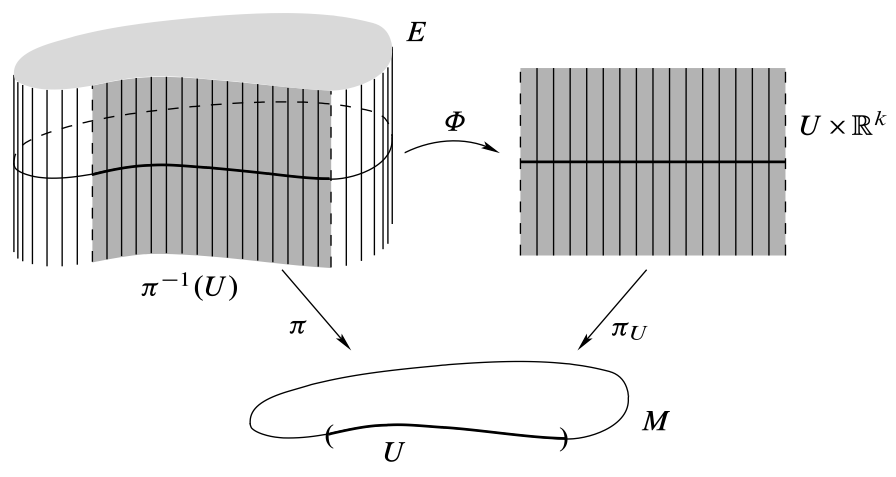
\includegraphics[width=300px]{vectorbundles_lee.png}
    \end{center}
    \caption{A schematic view of a real vector bundle \cite{lee12}.}
    \label{fig:vector_bundle}
\end{figure}

This definition is quite a mouthful, so let's dissect it, keeping Fig.~(\ref{fig:vector_bundle}) in mind.
Informally, the vector bundle $E$ is formed simply by attaching an $r$-dimensional $k$-vector space to each point of the manifold $M$.
This is precisely part $(i)$ of the definition. It is important to note, however, that these fibers must be ``put together'' in a way
that makes the total space $E$ a manifold, i.e. $E$ locally has a nice description, much like manifolds are required to be locally affine.
This is precisely what the local trivializations in $(ii)$ are meant to enforce: a vector bundle must locally look like the direct product of
the base manifold $M$ with the vector space $k^r$. Globally, however, the structure of the vector bundle might be ``twisted'' in some fashion.
A good example to keep in mind is the (infinite) Mobius strip: locally, for some open set $U\in S^1$ one can describe it as $U\times\R^1$;
globally, though, it becomes clear that the Mobius strip is twisted and cannot be written as a direct product. In this vein,
we say that a vector bundle is \textbf{trivial} if there exists a smooth local trivialization of $E$ over all of $M$, i.e. a diffeomorphism from $E$
to the product $M\times k^r$.

It may be useful to think of local trivializations for vector bundles as analogous to charts for manifolds. Any bundle that is not trivial
will clearly require more than one local trivialization. Just as in the case for transition maps between charts of a manifold, the transitions
between smooth local trivializations are well-behaved, as shown in the following lemma.

\begin{lem}
    Let $\pi:E\to M$ be a smooth vector bundle of rank $r$ over $M$. Suppose $\Phi:\pi^{-1}(U)\to U\times k^r$ and $\Psi:\pi^{-1}(V)\to V\times k^r$
    are two smooth local trivializations of $E$ with $U\cap V\neq\varnothing$. Then there exists a smooth map $\tau:U\cap V\to GL_r(k)$
    such that the composition $\Phi\circ\Psi^{-1}:(U\cap V)\times k^r\to (U\cap V)\times k^r$ has the form
    \[\Phi\circ\Psi^{-1}(p,v)=\left( p,\tau(p)v \right)\]
    where $\tau(p)v$ denotes the usual action of the $r\times r$ matrix $\tau(p)$ on the vector $v\in k^r$.
\end{lem}
\begin{proof}
%    By the definition of a vector bundle, the following diagram commutes:
%    \begin{equation*}
%        \begin{tikzcd}
%            (U\cap V)\times k^r\arrow{rd}[swap]{\pi_1} &\pi^{-1}(U\cap V)\arrow{l}[swap]{\Psi}\arrow{r}{\Phi}\arrow{d}[swap]{\pi} & (U\cap V)\times k^r\arrow{ld}{\pi_1}\\
%            & U\cap V, & 
%        \end{tikzcd}
%    \end{equation*}
%    where the maps on top are to be interpreted as restrictions of $\Psi$ and $\Phi$ to $\pi^{-1}(U\cap V)$.
    See \cite{lee12}, chapter 10.
\end{proof}

This simply means that the transition function between two local trivializations takes fiber to fiber as a linear isomorphism.
Consider again the example of the M\"obius strip; seen as a line bundle over the circle, we can take an open cover for $S^1$ to
be the usual two north/south-pole stereographic charts. On the circle, these charts overlap about the east/west-poles, and thus there
are two transition functions: on one of the regions $\tau(p)=-1$, and on the other, $\tau(p)=+1$. It is precisely this $-1$ that
``flips'' one of the attached $\R^1$ fibers to give the characteristic M\"obius twist.


The transition functions associated with the vector bundle carry quite a bit of information, as the following theorem shows.

\begin{thm}
    Suppose $M$ is a manifold with open cover $\{U_\alpha\}_{\alpha\in A}$. Suppose for each $\alpha,\beta\in A$ we are given
    a smooth map $\tau_{\alpha\beta}:U_\alpha\cap U_\beta\to \text{GL}(r,k)$ such that the \textbf{cocycle condition}
    \[\begin{array}[]{cc}
            \tau_{\alpha\beta}(p)\tau_{\beta\gamma}(p)=\tau_{\alpha\gamma}(p),&p\in U_\alpha\cap U_\beta\cap U_\gamma
        \end{array}
    \]
    is satisfied for all $\alpha,\beta,\gamma\in A$. Then there exists a smooth rank-$r$ vector bundle $E\to M$ with smooth local trivializations
    $\Phi_\alpha:\pi^{-1}\left( U_\alpha \right)\to U_\alpha\times k^r$ whose transition functions are the given maps $\tau_{\alpha\beta}$.
\end{thm}
\begin{proof}
    Left as an exercise to the reader. Hint: consider the disjoint union $\coprod_{\alpha\in A}\left( U_\alpha\times k^r \right)$ and define
    an appropriate equivalence relation. Quotienting by this equivalence relation should yield a vector bundle.
\end{proof}


This fact is quite useful, as we will see in the next section.

It should be clear that the tangent bundle that we discussed in the previous section is a prime example of a vector bundle. The vector spaces
comprising the bundle are simply the tangent spaces to the manifold; the open cover and the transition functions follow in a straightforward manner
from those for the base manifold. Incidentally, we can take smooth vector fields as a motivating example and talk about smooth sections over a general vector
bundle, which turns out to be quite useful. The study of Riemannian geometry, for example, is the study of Riemannian metrics on manifolds, which are smooth symmetric
positive-definite two-tensor fields, i.e. smooth sections of a ``tensor'' (vector) bundle.

%Now that we can talk about vector bundles in general, we can also talk about maps between them. Let $\pi:E\to M$ and $\pi: E'\to M'$
%be vector bundles. Then a smooth map $F:E\to E'$ is called a \textbf{smooth bundle homomorphism} if there exists a smooth map $f:M\to M'$ such
%that the diagram
%\begin{equation*}
%    \begin{tikzcd}
%        E\arrow{r}{F}\arrow{d}[swap]{\pi} & E'\arrow{d}{\pi'}\\
%        M\arrow{r}[swap]{f} & M'
%    \end{tikzcd}
%\end{equation*}
%commutes and such that for each $p\in M$, the restricted map $F|_{E_p}:E_p\to E'_{f(p)}$ is linear (i.e. linear on fibers). Given such a diagram, we typically say that
%$F$ covers $f$. A bijective bundle homomorphism that is also a diffeomorphism is called a \textbf{smooth bundle isomorphism}.

It turns out that we can actually
use given vector bundles to produce new bundles! Indeed, most operations valid for vector spaces can be extended to vector bundles by performing the vector space
operations fiberwise. Given vector bundles $E\to M, F\to M$, for example, we can define the dual bundle $E^*$, which has fibers $(k^r)^*$ at each point,
or the direct sum bundle, which is a vector bundle $E\oplus F$ whose fibers at a point $p$ are $E_p\oplus F_p$, or the tensor product bundle $E\otimes F$ given by the
fiberwise tensor product, etc. \cite{hatchervectorbundles} We will see some of these constructions in action in the next section.


\section{Holomorphic line bundles over $\CP^1$}

Let us now turn to line bundles over $\CP^1$. This case is especially interesting because the line bundles over $\CP^1$ form a group
isomorphic to $(\Z,+)$! We will not prove this here, but let us see why this is at least plausible.

The complex projective line is defined as $\C^2-(0,0)/\sim$ where $(z_1,z_2)\sim (\lambda z_1,\lambda z_2)$ for $\lambda\in\C^\times$. In other words, $\CP^1$
is the space of one-dimensional subspaces of $\C^2$. Thus a natural vector bundle over $\CP^1$ is the \textbf{tautological bundle}:
to each point $p$ of $\CP^1$ attach the one-dimensional subspace associated to $p$ as a fiber. This yields a line bundle that is typically
denoted $\mathcal{O}(-1)$. 
Let us denote the usual charts for $\CP^1$ as $U_1,U_2$, where points in $\CP^1$ are written $[z_1:z_2]$ with $z_1\neq 0$ in $U_1$
and $z_2\neq 0$ in $U_2$. We can now compute the transition function $\tau_{12}:U_1\cap U_2\to\text{GL}(\C)$. First note that we can construct
the local trivializations $\Phi_1$ as mapping $\left( [1:z], (\lambda, \lambda z) \right)\in\pi^{-1}(U_1)$ to $([1:z], \lambda)\in U_1\times\C$
and $\Phi_2$ as mapping $\left( [w:1], (\lambda w, \lambda) \right)\in\pi^{-1}(U_2)$ to $([w:1], \lambda)\in U_2\times\C$. Hence, we have that
\[\Phi_1\circ\Phi_2^{-1}\left( [w:1],\lambda \right)=\Phi_1\left( [1:w^{-1}], (\lambda w,\lambda) \right)=([1:w^{-1}],\lambda w).\]
From this we can read off that $\tau_{12}([1:z])=w=z^{-1}$.

Now, given the tautological line bundle $\mathcal{O}(-1)$, how can we produce more line bundles? The simplest construction is the dual bundle,
$\mathcal{O}(1)$, whose fibers are linear maps $\Hom(\C,\C)$ instead of $\C$. We could simply take the dual (transpose) of our transition function
from above -- this however, would give us the transition function from $U_1$ to $U_2$, as dualizing maps flips the domain and codomain. Hence, we also have
to throw in an inverse to get $\tau^*_{12}([1:z])=w^{-1}=z$. This now sheds some light on the notation $\mathcal{O}(\pm 1)$ that we've been using, and in
the context of having an integers' worth of line bundles over $\CP^1$, it is natural to ask whether we can construct bundles with transition function
$z^n$ for $n\in\Z$ and if so, whether we can describe them nicely.

It should be clear that the trivial bundle $\mathcal{O}(0)$ has transition function $\tau_{12}=z^0=\id$. The next question to address is:
how do we construct $\mathcal{O}(-2)$? The answer, it turns out, is through tensor products. Given two copies of $\mathcal{O}(-1)$,
consider the tensor product $\mathcal{O}(-1)\otimes\mathcal{O}(-1)$ as a vector bundle over $\CP^1$ whose fibers are $\C\otimes\C$. The transition
function is now given by the tensor product of the transition functions of the individual bundles: $\tau^{\otimes 2}_{12}([1:z])=w\otimes w=w^2=z^{-2}$.
Thus we see that $\mathcal{O}(-2)=\mathcal{O}(-1)^{\otimes 2}$. More generally, it is easy to see that $\mathcal{O}(n)$ can be constructed 
by repeated tensor products of $\mathcal{O}(\pm 1)$.

If we take on faith that these are the only line bundles over $\CP^1$ (upto bundle isomorphism), we see that line bundles over $\CP^1$ form an abelian
group under the tensor product that is isomorphic to $(\Z,+)$.

Now that we know what the line bundles over $\CP^1$ look like, we might inquire as to what the holomorphic sections of the bundle look like. In this
case, a local section of $\mathcal{O}(n)$ simply associates each point $p$ in $U_i\subset\CP^1$ with a complex number in the fiber of $\mathcal{O}(n)$ above $p$.
Explicitly constructing local holomorphic sections is not particularly difficult: $U_i$ is homeomorphic to a subset of $\C$ and thus the problem reduces to constructing
a holomorphic functions on a subset of $\C$. More subtle is the problem of constructing a global holomorphic section, i.e. a section that is defined and
holomorphic over the whole manifold $\CP^1$. If we construct our line bundles over the usual charts $U_i$, we have one overlap region $V=U_1\cap U_2$.
Using the magic of complex numbers we can construct a (local) holomorphic section over $U_2$, whose restriction to $V$ can be extended uniquely to
obtain a (hopefully) holomorphic section over $U_1$. 

Consider the case for $\mathcal{O}(1)$. Take, for example, the monomial $f_2(w)=w$ on $U_2$. On $U_1$, then, we get (via extension) the
function
\[f_1(z)=\tau_{12}(z)f_2(z^{-1})=z\cdot z^{-1}=1.\]
It's clear that $w$ is holomorphic on $U_2$ and $1$ is holomorphic on $U_1$
(and that they agree on $V$), and thus
that we have a global holomorphic section on $\CP^1$. We can do the same if we define the function $f_2(w)=1$, which extends to
\[f_1(z)=\tau_{12}(z)f_2(z^{-1})=z\cdot1=z.\]
We again obtain a global holomorphic section! Any other monomial, however, does not
induce a global holomorphic section. Since any holomorphic function can be written as a power series, we see that the only global holomorphic
sections on $\mathcal{O}(1)$ are polynomials $a_0+a_1z$ (or $a_0w+a_1$).
%It is easy to see that this space is isomorphic to the space of homogeneous polynomials in $w$ and $z$ of degree 1.

Similarly, for $\mathcal{O}(2)$, we can take $f_2(w)$ to be defined by $1,w,w^2$, which will extend to $f_1(z)$ being $z^2,z,1$ resp.
In general, then, the space of global holomorphic sections on $\mathcal{O}(n)$ for $n>0$ is simply the space of polynomials in $z$ (or $w$)
of degree upto $n$.
%More symmetrically, we can write this space of global holomorphic sections as homogeneous polynomials in $w$ and $z$ of degree 2.
%In general, then, the space of global holomorphic sections on $\mathcal{O}(n)$ for $n>0$ is simply isomorphic to the space of homogeneous polynomials
%in $w$ and $z$ of degree $n$.
But what about if $n\leq 0$?  Well the trivial bundle, $\mathcal{O}(0)=\CP^1\times\C$, is easy. Global holomorphic sections simply correspond to holomorphic
functions $f:\CP^1\to\C$, which are constants (Liouville's theorem). Next consider $n=-1$, i.e. $\mathcal{O}(-1)$, which has transition function
$\tau_{12}(z)=z^{-1}$. Does $f_2(w)=1$ extend holomorphically to a global section? The usual calculation shows that
\[f_1(z)=\tau_{12}(z)f_2(z^{-1})=z^{-1},\]
which blows up at $[1:0]$, and is thus not holomorphic. Furthermore, if $f_2(w)=w$ we get
\[f_1(z)=\tau_{12}(z)f_2(z^{-1})=z^{-2},\]
which is clearly no good either. Indeed, it is easy to see that there is no holomorphic monomial in $w$ that extends to a holomorphic 
monomial in $z$, and hence there are no non-trivial global sections of $\mathcal{O}(-1)$. The same holds for all $\mathcal{O}(n)$ with
$n\leq -1$.

In conclusion, the space of global holomorphic sections of $\mathcal{O}(n)$ is trivial for negative $n$, and 
isomorphic to $\C^{n+1}$ for non-negative $n$. That we can explicitly determine these spaces of sections is a good measure of our understanding
of the bundles $\mathcal{O}(n)$. This understanding for line bundles in general, in fact, turns out to be very useful in representation theory
(the Borel-Weil-Bott theorem) and algebraic geometry (the line bundles over a variety yield information about the codimension 1 subvarieties).





\newpage

\bibliography{notes}
\bibliographystyle{alpha}

\end{document}
